\newpage
\section{Metodología}
Para la realización del Trabajo Terminal se utilizará una metodología híbrida compuesta por la metodología SCRUM que adopta el ciclo de vida de desarrollo de sistemas de cascada.

Las metodologías híbridas son una combinación de dos metodologías y retoman las ventajas de los dos tipos de metodologías lo que nos ayuda a formar una combinación de las mejores prácticas existentes dentro de ellas.

La metodología SCRUM es una metodología ágil y es altamente flexible, ya que la lista de sprints pueden ser modificadas en el transcurso del desarrollo del proyecto por diversos motivos que se tengan. Otro punto de SCRUM es que al trabajar por partes pequeñas y comenzar por las más importantes, es más fácil poder detectar problemas a futuro que tal vez puedan presentarse\cite{Referencia17}.

''Scrum es un proceso en el que se aplican de manera regular un conjunto de buenas prácticas para trabajar colaborativamente, en equipo, y obtener el mejor resultado posible de un proyecto. Estas prácticas se apoyan unas a otras y su selección tiene origen en un estudio de la manera de trabajar de equipos altamente productivos."\cite{Referencia18}

Uno de los beneficios de la metodología SCRUM es que los proyectos pueden ser entregados con una mejor calidad, ya que como es más fácil detectar problemas, estos pueden ser corregidos en el momento justo, antes de que seán más costosos y difíciles de corregir. 

En la figura \ref{fig:metodologiaSCRUM} se muestran las principales actividades abordadas por la metodología Scrum.
\newpage
\begin{figure}[htb]
	\centering
	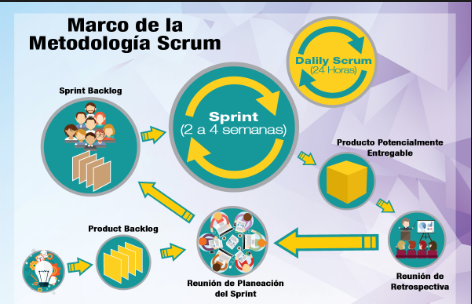
\includegraphics[width=1\textwidth]{images/introduccion/scrum}
	\caption{Marco de la Metodología SCRUM} \label{fig:metodologiaSCRUM}
\end{figure}

Se tendrán además prototipos de desarrollo donde se llevarán a cabo el análisis, diseño, construcción y pruebas de los prototipos implementados en cada etapa de la metodología anteriormente mencionada.\\

En cambio el modelo de desarrollo de sistemas de cascada, es un proceso de desarrollo secuencial, en el que el desarrollo de software se concibe como  un conjunto de etapas que  se ejecutan una tras otra. Se le denomina así por las posiciones que ocupan las diferentes fases que componen el proyecto, colocadas una encima de otra, y siguiendo un flujo de ejecución de arriba hacia abajo, como una cascada.\cite{Referencia21}

En la figura \ref{fig:cascada} se muestran las principales actividades abordadas por el modelo de desarrollo de sistemas de cascada.
\newpage
\begin{figure}[htb]
	\centering
	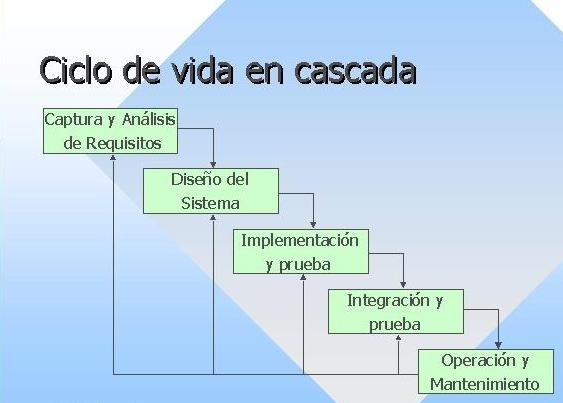
\includegraphics[width=1\textwidth]{images/cap2/cascada}
	\caption{Modelo de Desarrollo de Sistemas de Cascada} \label{fig:cascada}
\end{figure}

Para poder trabajar con esta metodología híbrida manejaremos un ciclo de vida de desarrollo de sistemas de cascada dentro de cada sprint de SCRUM.

Esta metodología híbrida será aplicada a nuestro Trabajo Terminal de la siguiente manera:\\

\textbf{Trabajo Terminal 1}
Se trabajarán los primeros 2 sprints para esta primer parte del Trabajo Terminal
\begin{itemize}
	 
	\item El sprint 1 constará de:
	\begin{itemize}
		\item Análisis de requerimientos.
		\item Análisis del Proceso
	\end{itemize}
	
	\item El sprint 2 constará de:
	\begin{itemize}
		\item Análisis formal del Rol del Paciente por medio de casos de uso.
		\item Diseño de Pantallas del Rol del Paciente por medio de Mockups
	\end{itemize}
\end{itemize}

\textbf{Trabajo Terminal 2}
Se trabajarán los últimos 3 sprints para esta última parte del Trabajo Terminal

\begin{itemize}
	\item El sprint 3 constará de:
	\begin{itemize}
		\item Análisis formal del Rol del Doctor por medio de casos de uso.
		\item Diseño de Pantallas del Rol del Doctor por medio de Mockups.
		\item Análisis formal del Rol del Auxiliar por medio de casos de uso.
		\item Diseño de Pantallas del Rol del Auxiliar por medio de Mockups.
	\end{itemize}
	\item El sprint 4 constará de:
	\begin{itemize}
		\item Desarrollo de los módulos correspondientes a los roles del Doctor y del Auxiliar.
	\end{itemize}
	\item El sprint 5 constará de:
	\begin{itemize}
		\item Pruebas Técnicas de cada uno de los módulos que conforman la aplicación.
		\item Pruebas de Usuarios de cada uno de los módulos que conforman la aplicación.
	\end{itemize}
\end{itemize}

En la figura \ref{fig:arquitectura3} se definen los módulos trabajados para Trabajo Terminal 1 y los módulos trabajados para Trabajo Terminal 2. 

\begin{figure}[htb]
	\centering
	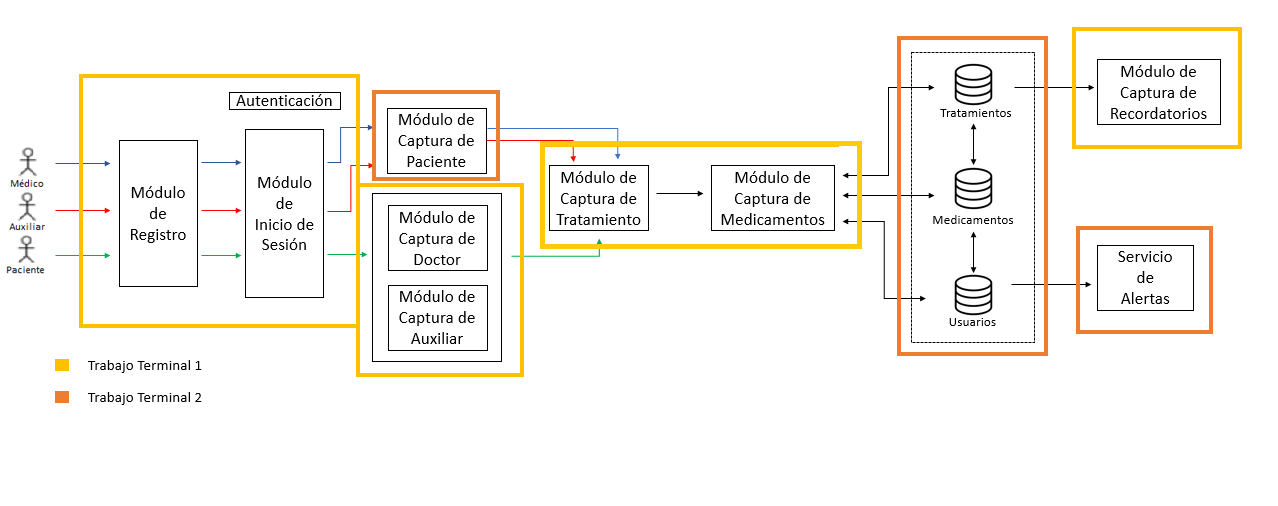
\includegraphics[width=1\textwidth]{images/cap2/Arquitectura3_1}
	\caption{TT1 y TT2} \label{fig:arquitectura3}
\end{figure}

%\textbf{Trabajo Terminal 2}
%\begin{itemize}
%	\item Se trabajarán los últimos 3 sprints para esta segunda parte del Trabajo Terminal.
%	\item El sprint 3 constará de la definición formal de la aplicación.
%	\item El sprint 4 constará del diseño del sistema, diseño de pantallas por medio de mockups e implementación de los prototipos restantes que en este caso, serán las partes de los roles del \textbf{Doctor} y el \textbf{Auxiliar}.
%	\item El sprint 5 constará de las pruebas de la aplicación, la generación del manual de usuario y la generación del reporte técnico para la entrega final del Trabajo Terminal.
%\end{itemize}

\newpage
\section{Arquitectura}

En la figura \ref{fig:arquitectura1} se muestra el diagrama de la arquitectura propuesta con la que se trabajará para solucionar la problemática.

%En la figura \ref{fig:arquitectura} se describirá la arquitectura propuesta para la solución de la problemática.

\begin{figure}[htb]
	\centering
	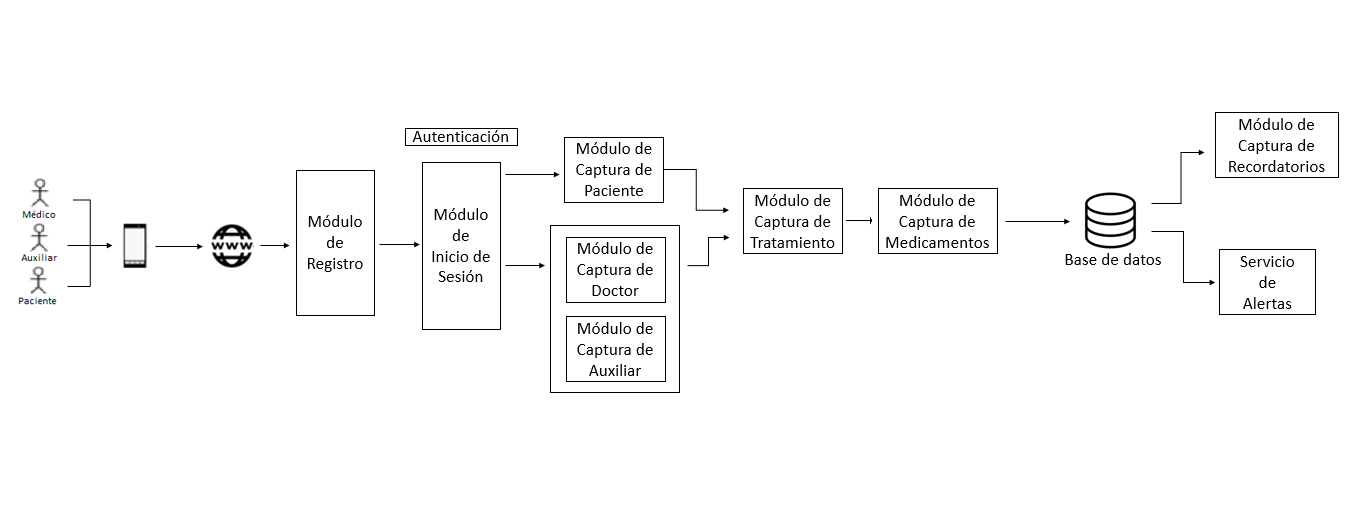
\includegraphics[width=1\textwidth]{images/cap2/Arquitectura4_1}
	\caption{Arquitectura} \label{fig:arquitectura1}
\end{figure}

Como podemos notar en la figura \ref{fig:arquitectura1} se cuenta con tres roles que participarán en el sistema, los cuales son :
\begin{itemize}

	\item Paciente: Se le llama paciente a la persona que cuenta con un tratamiento generado por el médico que se encuentra a cargo de su salud.\\
	
	Las acciones con las que cuenta su rol son:
	\begin{itemize}
		\item Consultar sus tratamientos médicos.
		\item Agregar el tratamiento médico.
		\item Agregar medicina a tratamiento médico.
		\item Modificar el tratamiento médico.
		\item Modificar medicamentos.
		\item Eliminar medicamentos.
		\item Consultar tomas del medicamento.
		%		\item Eliminar el tratamiento médico.
%		\item Agregar doctor
		\item Consultar doctor.
		%		\item Asociar doctor.
%		\item Eliminar doctor.
		\item Consultar auxiliares.
		\item Agregar auxiliar.
		%		\item Asociar auxiliar.
		\item Eliminar auxiliar.
		%		\item Agregar contactos de emergencia
		%		\item Consultar contactos de emergencia.
		%		\item Asociar contacto de emergencia.
		%		\item Eliminar contacto de emergencia.
		%		\item Editar recordatorios.
		\item Consultar recordatorios.
		%		\item Consultar alertas.
		\item Consultar sus datos personales.
		\item Editar sus datos personales.
	\end{itemize}

	\item Doctor: \textbf{Doctor} dentro del sistema es el profesional de la salud que se encarga del diagnóstico del paciente.
	Las acciones con las que cuenta su rol son:
		\begin{itemize}
			
			\item Consultar pacientes.
			\item Consultar tratamiento médico de pacientes.
			\item Modificar tratamiento médico de pacientes.
			\item Eliminar tratamiento médico de sus pacientes.
			\item Agregar paciente nuevo.
%			\item Asociar nuevo paciente.
			\item Agregar tratamiento médico.
			\item Agregar medicina a tratamiento médico.
%			\item Editar notificaciones.
%			\item Consultar historial clínico.
%			\item Eliminar paciente.
%			\item Editar paciente.
			\item Consultar sus datos personales.
			\item Editar sus datos personales.
			
		\end{itemize}

	\item Auxiliar: nace de la necesidad de ayudar a los pacientes que cuentan con poca o nula experiencia los dispositivos móviles o que por factores ajenos a la aplicación como son la edad o alguna enfermedad, les sea imposible utilizar la aplicación por si mismos\\
	Las acciones con las que cuenta su rol son:
	\begin{itemize}
		
		
		\item Agregar paciente.
		\item Eliminar paciente.
%		\item Editar paciente.
		\item Consultar tratamiento médico de paciente.
		\item Agregar tratamiento médico de paciente.
		\item Agregar medicina a tratamiento médico.
%		\item Modifica tratamientos.
		\item Eliminar tratamiento médico de paciente.
%		\item Editar sus notificaciones.
%		\item Agregar doctor
		\item Consultar doctor.
%		\item Eliminar doctor
%		\item Asociar doctor.
%		\item Agregar contactos de emergencia
%		\item Consultar contactos de emergencia.
%		\item Eliminar contacto de emergencia.
		\item Consultar recordatorios.
%		\item Consultar alertas.
		\item Consultar sus datos personales.
		\item Editar sus datos personales.
%		
%		\item Agregar Paciente.
%		\item Modificar Paciente.
%		\item Eliminar Paciente.
%		\item Agregar Tratamiento medico.
%		\item Modificar Tratamiento medico.
%		\item Consultar Tratamiento medico.
%		\item Modificar notificación
	\end{itemize}
\end{itemize}


\section{Módulos}
La arquitectura contará con los siguientes módulos:
\begin{itemize}
	\item Módulo de Registro: Este módulo es el encargado de registrar e ingresar a los actores dentro de la aplicación. 
	
	
	\item Módulo de Autenticación: Una vez que te hayas registrado dentro de la aplicación, el módulo de autenticación se encargará de verificar tu usuario y habilitar los módulos correspondientes a tu rol.
	
	\item Módulo de Inicio de Sesión: Este módulo te permitirá ingresar a los módulos correspondientes a tu rol ingresando con tu usuario y contraseña previamente registrados e el Módulo de Registro.
	
	 
	\item Módulo de Captura de Paciente: Este módulo es el encargado de agregar al paciente con el que trabajarán el doctor y el auxiliar.
	
	\item Módulo de Captura de Doctor: Este módulo es el encargado de agregar al doctor que está a cargo del tratamiento del paciente.
	
	\item Módulo de Captura de Auxiliar: Este módulo es el encargado de agregar al auxiliar que está a cargo del tratamiento del paciente.
	
%	\item Módulo de Captura de Contactos de Emergencia:Este módulo es el encargado de agregar los contactos de emergencia que podrán recibir las alertas del paciente que los haya agregado.
	
	\item Módulo de Captura de Tratamiento: Este módulo es el encargado de ingresar el tratamiento médico del paciente y con el que podrán trabajar tanto el doctor como el auxiliar. 
%	y lo asociara al perfil del paciente con la información correspondiente del tratamiento.

	\item Módulo de Captura de Medicamentos: Este módulo es el encargado de ingresar los medicamentos que son recetados por el Doctor para que el paciente siga su tratamiento médico.
	
	\item Módulo de Recordatorios: Este módulo es el encargado de crear los recordatorios de las medicinas una vez que éstas hayan sido ingresadas dentro del tratamiento médico.
	
	\item Módulo de Servicio de Alertas: Este módulo es el encargado de mandar las notificaciones al usuario.
	
%	\item Módulo de Alertas: Este módulo es el encargado de crear las alarmas cuando un medicamento sea de alta prioridad y que si no se toma en el momento, pueda tener efectos negativos en el paciente.
	
%	\item Módulo de Reportes: Este módulo es el encargado de generar un reporte con la información del tratamiento y datos relevantes del paciente como lo son la edad, estatura, peso, etc.
	
	
	
	
	
%	\item Módulo de Autenticación: El modulo encargado de verificar tu perfil y darte acceso a los módulos correspondientes.
%	\item Módulo captura de tratamientos: El modulo encargado de ingresar el tratamiento medico y lo asociara al perfil del paciente con la información correspondiente del tratamiento.
%	\item Módulo de recordatorios: Una vez que se paso por el modulo de \textbf{Captura de tratamiento} llegamos al modulo de recordatorios en donde se generaran los notificaciones a partir de la información obtenida del modulo de captura de tratamiento.
%	\item Módulo de alarmas: Este modulo es el encargado de cuando una notificación no haya sido silenciada esta se convierta en una alarma que le estará recordando al paciente tomar su medicamento.
%	\item Módulo de reportes: El modulo de reportes sirve para notificar al medico y al paciente que tan constante ha sido con su tratamiento.
%	\item Módulo de estadísticas: 
\end{itemize}
\newpage
\section{Modelo Relacional}
En la siguiente figura \ref{fig:modelorelacional} se muestra el modelo relacional con el que trabajará la aplicación mostrando así los datos que estarán proporcionando cada una de las partes responsables para que funcionen de manera correcta todos los módulos.

\begin{figure}[htb]
	\centering
	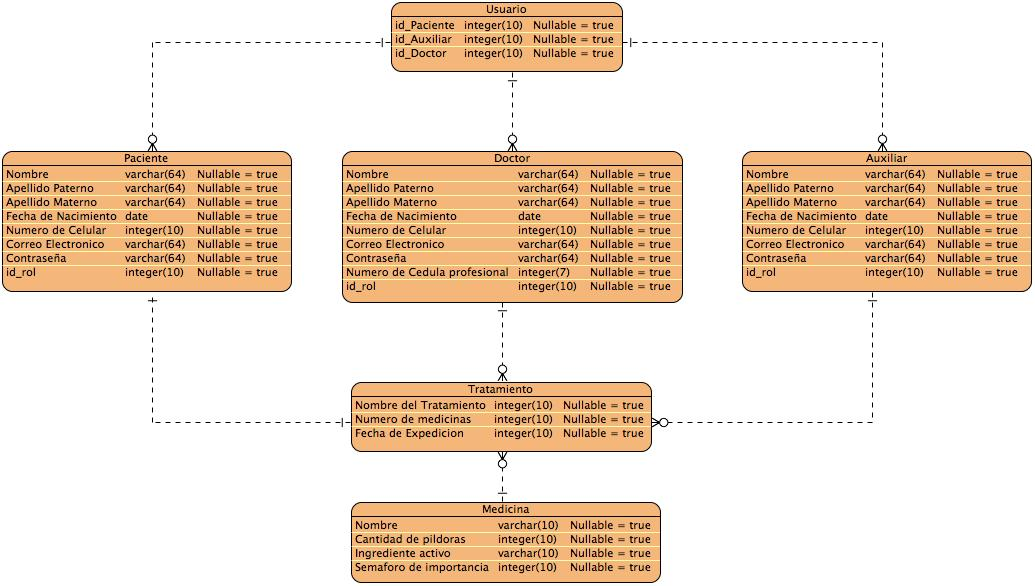
\includegraphics[width=1.1\textwidth]{images/cap2/modelorelacional}
	\caption{Modelo Relacional de Rem-Pills} \label{fig:modelorelacional}
\end{figure} 




\section{Requerimientos}
Los requerimientos funcionales describen lo que el sistema debe hacer. Son declaraciones de los servicios que debe proporcionar el sistema, de la manera en que éste debe reaccionar a entradas particulares y de cómo se debe comportar en situaciones particulares.\\
En la siguiente sección se especificarán los requerimientos con los que estará trabajando la aplicación.\\
%\begin{itemize}
%		\item RF1 - Registro de Usuario
%		La aplicación permitirá el registro de nuevos usuarios mediante el ingreso de su nombre, correo electrónico y contraseña.
%		
%		\item RF2 - Acceso al Sistema.
%		La aplicación permitira el acceso al sistema proporcionando el correo electrónico y la contraseña con la que se registraron en la aplicación
%		
%		Los usuarios accederán al sistema proporcionando el correo electrónico y la contraseña con la que se registraron en la aplicación
%		
%		\item RF3 - Agregar Paciente.
%		 
%		 La aplicación permitirá que tanto el doctor como el auxiliar agreguen a los pacientes con los que están trabajando a la \textbf{lista de pacientes}.
%		 
%		El usuario doctor agregará a un paciente a su \textbf{lista de pacientes} ingresando el correo electrónico o nombre del paciente.
%		El usuario auxiliar agregará a un paciente a su \textbf{lista de pacientes} ingresando el correo electrónico o nombre del paciente.
%		El usuario paciente agregará a un doctor a su \textbf{lista de doctores} ingresando el correo electrónico o nombre del paciente.
%		El usuario paciente agregará a un doctor a su \textbf{lista de auxiliares} ingresando el correo electrónico o nombre del paciente.
%	
%		\item RF4 - Agregar Doctor o Auxiliar.
%		
%		La aplicación permitirá al Paciente agregar al doctor que receto su tratamiento a su \textbf{lista de doctores} y en el caso de que sea necesario, agregar a la \textbf{lista de auxiliares} a un auxiliar para que sea el encargado de su tratamiento.
%		
%%		\item RF5 - Alta de Invitación.
%%		
%%		Cuando un usuario haya agregado a otro usuario, la aplicación mandará un correo con el cual se vincularán sus perfiles.
%		
%		\item RF6 - Agregar Tratamiento.
%		
%		La aplicación permitirá  ya sea al doctor, auxiliar o paciente agregar el tratamiento expedido por el doctor al perfil del paciente en cuestión.
%		
%		\item RF7 - Creación de Recordatorios.
%		
%		La aplicación creará los recordatorios de los medicamentos a tomar  una vez que el tratamiento haya sido ingresado en el sistema.
%		
%		\item RF8 - Creación de Alarmas.
%		
%		La aplicación permitirá al usuario configurar alarmas cuando el ingerir un medicamento sea de suma importancia.
%		
%		\item RF9 - Gestión de Contactos de Emergencia.
%		
%		Cuando una notificación de un medicamento con un alta importancia no haya sido silenciada después de tres intentos, la aplicación mandará un mensaje a los contactos de emergencia.
%		
%		\item RF10 - Creación de reportes.
%		
%		La aplicación permitirá al usuario ingresar datos relevantes de su salud y creará un reporte con el avance de sus tratamientos los datos ingresados.
%\end{itemize}
%
%
%Requerimientos No Funcionales
%\begin{itemize}
%	\item RNF-1 Creación de Usuario
%	La creación del usuario dependerá del rol que tenga, esto quiere decir que el formulario que llenará un doctor es distinto al de un paciente.
%	
%	\item RNF-2 Verificación de Perfil
%	La aplicación distinguirá entre los 4 tipos de roles que hay, los cuales son: Paciente, Auxiliar, Doctor y Administrador.
%	
%	\item RNF-3 Recordatorios.
%	Un recordatorio esta compuesto por un mensaje que se desplegara en la pantalla y que al llegar generara un sonido, notificando que es tiempo de tomar el medicamento.
%	
%	\item RNF-4 Interfaz Comprensible.
%	La aplicación contará con iconos, botones y formularios que muestran de forma clara lo que hace cada uno y con datos que se consiguen de la receta que expide el medico o que viene en la caja del medicamento.
%	
%	\item RNF-5 Base de datos.
%	La aplicación contará con una base de datos de forma local que permitirá que la consulta de los datos sea más rápida.
%	
%	\item RNF-6 Desarrollo Multiplataforma.
%	La aplicación sera desarrollada para los sistemas operativos iOS y Android de forma nativa permitiendo así explotar todas sus ventajas.
%	
%	\item RNF-7 Desempeño Web y Móvil.
%	La aplicación permitirá que el registro del tratamiento sea ingresado por una servicio web o mediante la aplicación móvil. 
%	
%	\item RNF-8	Protección de Información
%	La aplicación contará con un cifrado AES-128 para proporcionar toda la seguridad a la información del usuario.
%\end{itemize}





\begin{ReqUser}		
	\reqUserItem{RF1}{Registro de Usuario}{
		El usuario requiere de un mecanismo que le permita registrarse en la aplicación.
	}
	{\alta}{}{\corregir}
\end{ReqUser}

\begin{ReqUser}		
	\reqUserItem{RF2}{Acceso al Sistema}{
		El usuario requiere de un mecanismo que le permita ingresar al sistema.
	}
	{\alta}{}{\corregir}
\end{ReqUser}


%	\begin{ReqUser}		
%		\reqUserItem{RF3}{Recuperar Contraseña}{
%			El usuario requiere de un mecanismo que le permita recuperar su contraseña o crear una contraseña nueva.
%		}
%		{\alta}{}{\corregir}
%	\end{ReqUser}

\begin{ReqUser}		
	\reqUserItem{RF3}{Agregar Paciente}{
		El doctor y el auxiliar requieren de un mecanismo que le permita agregar a un nuevo paciente.
	}
	{\alta}{}{\corregir}
\end{ReqUser}

\begin{ReqUser}		
	\reqUserItem{RF4}{Agregar Doctor}{
		El paciente requiere de un mecanismo que le permita agregar a un doctor.
	}
	{\alta}{}{\corregir}
\end{ReqUser}


\begin{ReqUser}		
	\reqUserItem{RF5}{Agregar Auxiliar}{
		El paciente requiere de un mecanismo que le permita agregar a un auxiliar.
	}
	{\alta}{}{\corregir}
\end{ReqUser}

%	\begin{ReqUser}		
%		\reqUserItem{RF7}{Agregar Contactos de Emergencia}{
%			El paciente requiere de un mecanismo que le permita agregar a un contacto de emergencia.
%		}
%		{\alta}{}{\corregir}
%	\end{ReqUser}

\begin{ReqUser}		
	\reqUserItem{RF6}{Agregar Tratamiento}{
		El usuario requiere de un mecanismo que le permita agregar un nuevo tratamiento.
	}
	{\alta}{}{\corregir}
\end{ReqUser}

\begin{ReqUser}		
	\reqUserItem{RF7}{Agregar Medicina}{
		El usuario requiere de un mecanismo que le permita agregar una medicina nueva a un tratamiento.
	}
	{\alta}{}{\corregir}
\end{ReqUser}

\begin{ReqUser}		
	\reqUserItem{RF8}{Consultar Tratamiento}{
		El usuario requiere de un mecanismo que le permita consultar la información de su tratamiento.
	}
	{\alta}{}{\corregir}
\end{ReqUser}

\begin{ReqUser}		
	\reqUserItem{RF9}{Consultar Doctores}{
		El usuario requiere de un mecanismo que le permita consultar la información de sus doctores.
	}
	{\alta}{}{\corregir}
\end{ReqUser}

\begin{ReqUser}		
	\reqUserItem{RF10}{Consultar Auxiliares}{
		El usuario requiere de un mecanismo que le permita consultar la información de sus auxiliares.
	}
	{\alta}{}{\corregir}
\end{ReqUser}

\begin{ReqUser}		
	\reqUserItem{RF11}{Recordatorios}{
		La aplicación creara los recordatorios para los medicamentos en un tratamiento médico.
	}
	{\alta}{}{\corregir}
\end{ReqUser}

%	\begin{ReqUser}		
%		\reqUserItem{RF14}{Alarmas}{
%			La aplicación creará las alarmas para los medicamentos que sean de suma importancia en el tratamiento del paciente.
%		}
%		{\alta}{}{\corregir}
%	\end{ReqUser}

%	\begin{ReqUser}		
%		\reqUserItem{RF15}{Alarmas}{
%			La aplicación creará las alarmas para los medicamentos que sean de suma importancia en el tratamiento del paciente.
%		}
%		{\alta}{}{\corregir}
%	\end{ReqUser}

%	\begin{ReqUser}		
%		\reqUserItem{RF15}{Creación de Reportes}{
%			El usuario requiere de un mecanismo que genere un reporte con los datos de su perfil, sus doctores y sus auxiliares.
%		}
%		{\alta}{}{\corregir}
%	\end{ReqUser}

\begin{ReqUser}
	\reqSistItem{RF12}{Creación de Rol}
	{La aplicación creará al usuario dependiendo de los roles que éste seleccione.}{\alta}{}{\corregir}
\end{ReqUser}

\begin{ReqUser}
	\reqSistItem{RF13}{Verificación de Rol}
	{
		La aplicación verificará los roles que tiene el usuario y habilitará los módulos correspondientes.
	}
	{\alta}{}{\corregir}
\end{ReqUser}
\newpage


\textbf{Requerimientos No Funcionales}

	
%	\begin{ReqSist}
%		\reqSistItem{RNF1}{Creación de Rol}
%		{La aplicación creará al usuario dependiendo de los roles que éste seleccione.}{\alta}{\refUserReq{RF1},\refUserReq{RF2}}{}
%	\end{ReqSist}
%
%	\begin{ReqSist}
%		\reqSistItem{RNF2}{Verificación de Rol}
%		{
%			La aplicación verificará los roles que tiene el usuario y habilitará los módulos correspondientes.
%		}
%		{\alta}
%		{\refUserReq{RF1}\refUserReq{RF2}}{}
%	\end{ReqSist}

\begin{ReqSist}
	\reqSistItem{RNF1}{Creación de Recordatorios}
	{
		La aplicación creará los recordatorios de los medicamentos que pertenecen a un tratamiento una vez que estos hayan sido agregados.
	}
	{\alta}
	{\refUserReq{RU-MR1}}{}
\end{ReqSist}

%	\begin{ReqSist}
%		\reqSistItem{RNF2}{Creación de Alarmas}
%		{
%			La aplicación creará las alarmas cuando un medicamento cuente con una clasificación de \textbf{Importante} y éste haya sido agregado al tratamiento.
%		}
%		{\alta}
%		{\refUserReq{RU-MR1}}{}
%	\end{ReqSist}

\begin{ReqSist}
	\reqSistItem{RNF2}{Interfaz Comprensible}
	{
		La aplicación contará con íconos que expliquen su funcionalidad, los formularios preguntarán por datos que se encuentren en la receta expedida por el doctor o que se encuentren en la caja del medicamento.
	}
	{\alta}
	{\refUserReq{RU-MR1}}{}
\end{ReqSist}

\begin{ReqSist}
	\reqSistItem{RNF3}{Foto de Perfil}
	{
		La aplicación contará con 4 avatares que se podrán seleccionar en el caso de que el usuario no pueda realizar o seleccionar la foto de perfil en el momento en que está creando su cuenta.
	}
	{\alta}
	{\refUserReq{RU-MR1}}{}
\end{ReqSist}

\begin{ReqSist}
	\reqSistItem{RNF4}{Base de Datos}
	{
		La aplicación contará con una base de datos de forma local que permitirá que la consulta de los datos sea más rápida.
	}
	{\alta}
	{\refUserReq{RU-MR1}}{}
\end{ReqSist}

\begin{ReqSist}
	\reqSistItem{RNF5}{Desarrollo Multiplataforma}
	{
		La aplicación será desarrollada para los sistemas operativos iOS y Android de forma nativa para así explotar todas sus ventajas.
	}
	{\alta}
	{\refUserReq{RU-MR1}}{}
\end{ReqSist}

%	\begin{ReqSist}
%		\reqSistItem{RNF9}{Servicio Web}
%		{
%			La aplicación permitirá que el registro de un tratamiento sea ingresado por un servicio web.
%		}
%		{\alta}
%		{\refUserReq{RU-MR1}}{}
%	\end{ReqSist}

%	\begin{ReqSist}
%		\reqSistItem{RNF9}{Protección de Información}
%		{
%			La aplicación contará con un cifrado AES-128 para proporcionar la seguridad de la información del usuario.
%		}
%		{\alta}
%		{\refUserReq{RU-MR1}}{}
%	\end{ReqSist}



	


\section{Procesos}

En la siguiente sección se muestran los procesos de cómo es una consulta médica en la actualidad y cómo será una consulta médica con el uso de la aplicación.


En la figura \ref{fig:proceso1} con su subproceso \ref{fig:subproceso1} se muestra cómo se maneja en la actualidad las consultas médicas y por ende la expedición de los tratamientos médicos.

En cambio con el uso de la aplicación como se muestra en la imagen \ref{fig:proceso2} y su subproceso \ref{fig:subproceso2} podemos notar cómo el uso de las nuevas tecnologías ayuda tanto a los pacientes como a los médicos.

\newpage
\begin{landscape}
	
\begin{figure}[htb]
	\centering
	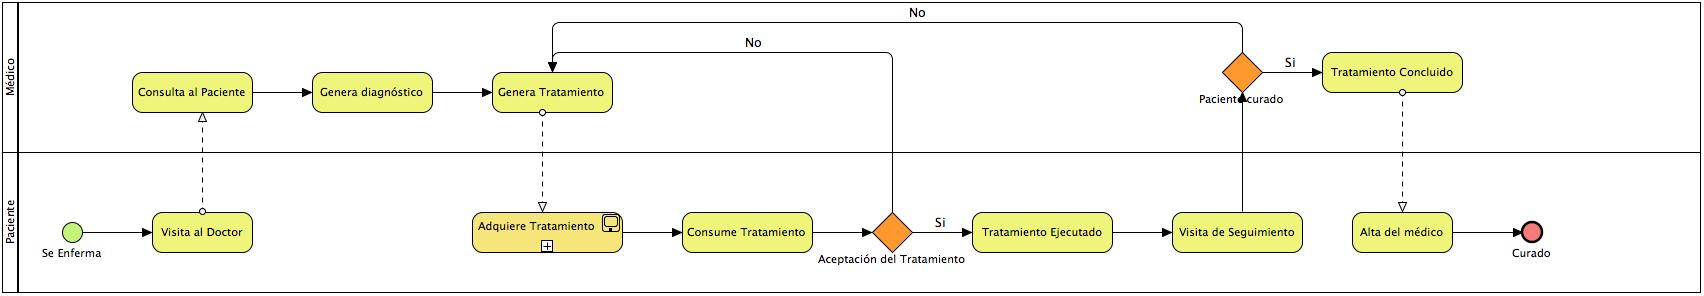
\includegraphics[width=1.5\textwidth]{images/cap2/Proceso1}
	\caption{Proceso médico en la actualidad} \label{fig:proceso1}
\end{figure}
\newpage

\begin{figure}[htb]
	\centering
	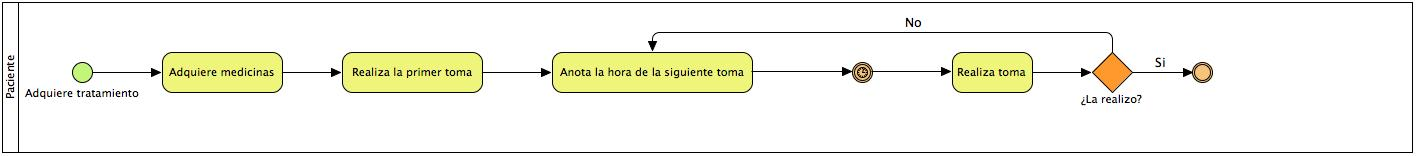
\includegraphics[width=1.5\textwidth]{images/cap2/AdquiereTratamientoP1}
	\caption{Sub-proceso Adquiere tratamiento en la actualidad} \label{fig:subproceso1}
\end{figure}
\newpage
\begin{figure}[htb]
	\centering
	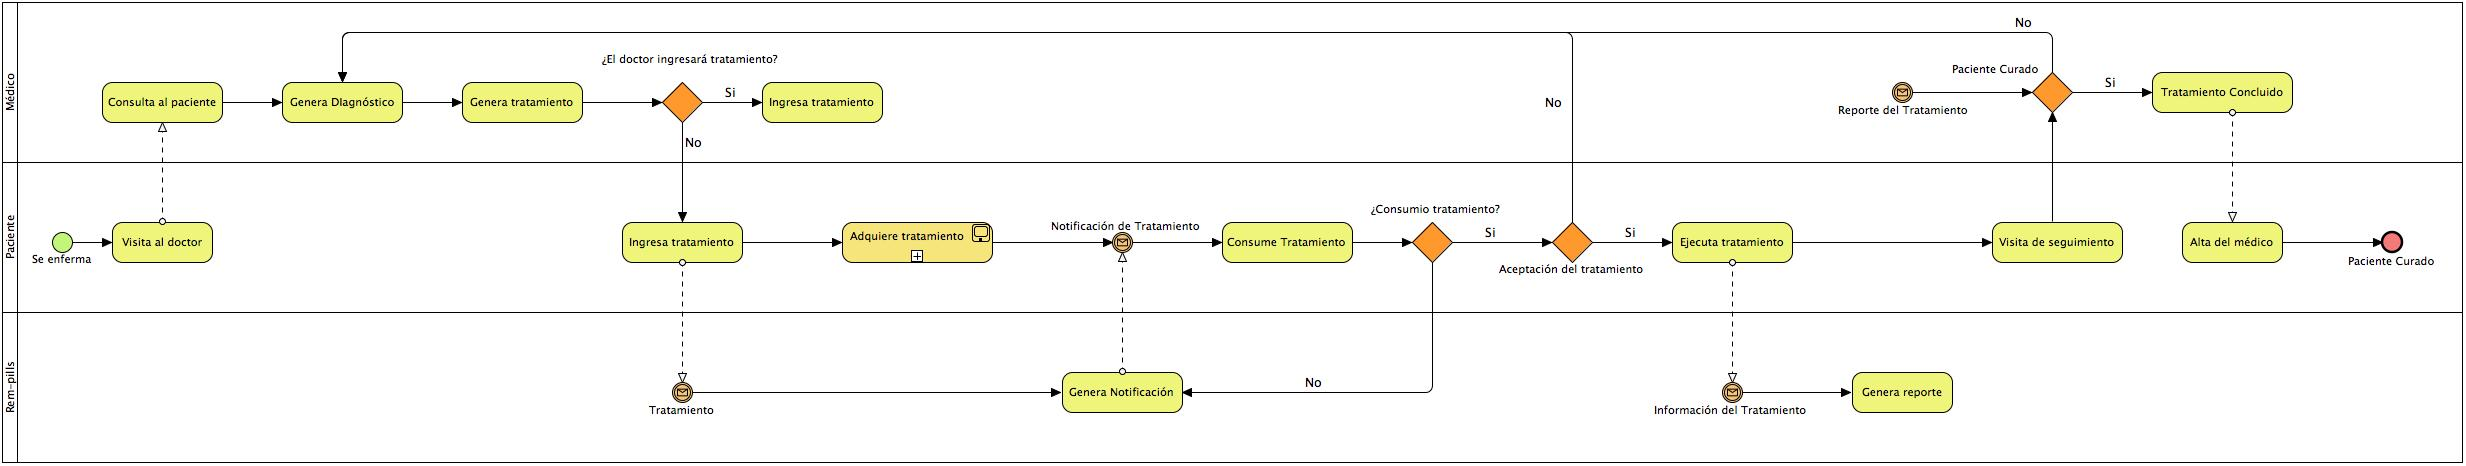
\includegraphics[width=1.5\textwidth]{images/cap2/Proceso2}
	\caption{Proceso médico con ayuda de la aplicación} \label{fig:proceso2}
\end{figure}
\newpage
\begin{figure}[htb]
	\centering
	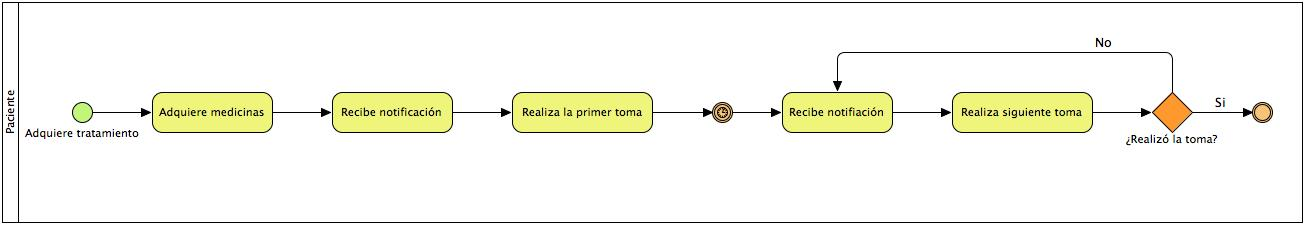
\includegraphics[width=1.5\textwidth]{images/cap2/AdquiereTratamientoP2}
	\caption{Sub-proceso Adquiere tratamiento con ayuda de la aplicación} \label{fig:subproceso2}
\end{figure}
\newpage
\begin{figure}[htb]
	\centering
	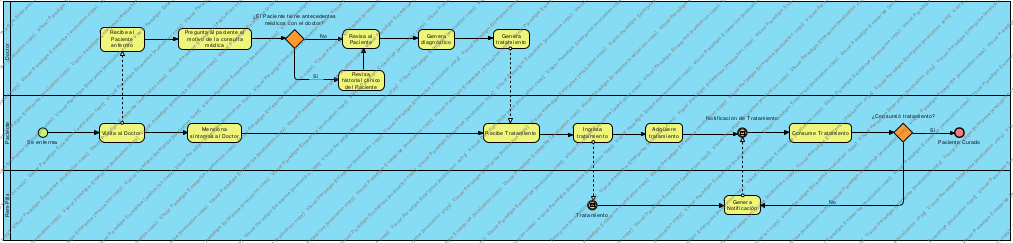
\includegraphics[width=1.5\textwidth]{images/cap2/ProcesosDoctor}
	\caption{Proceso del Doctor} \label{fig:proceso3}
\end{figure}
\newpage
\begin{figure}[htb]
	\centering
	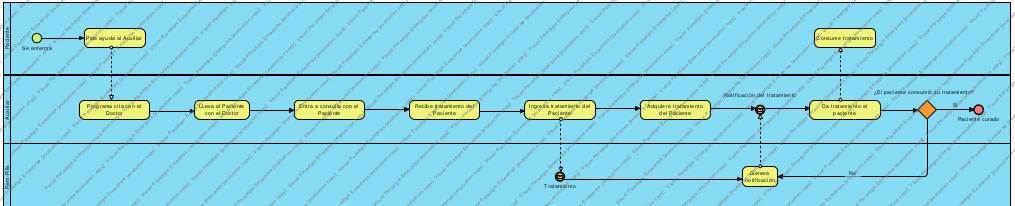
\includegraphics[width=1.5\textwidth]{images/cap2/ProcesosAuxiliar}
	\caption{Proceso del Auxiliar} \label{fig:proceso4}
\end{figure}

\end{landscape}



\section{Casos de uso}
En el análisis realizado para la aplicación Rem-Pills se identificaron los siguientes casos de uso como se muestra en las figuras \ref{fig:casosdeuso}, \ref{fig:casosdeusoD}, \ref{fig:casosdeusoA}\\

\begin{figure}[htb]
	\centering
	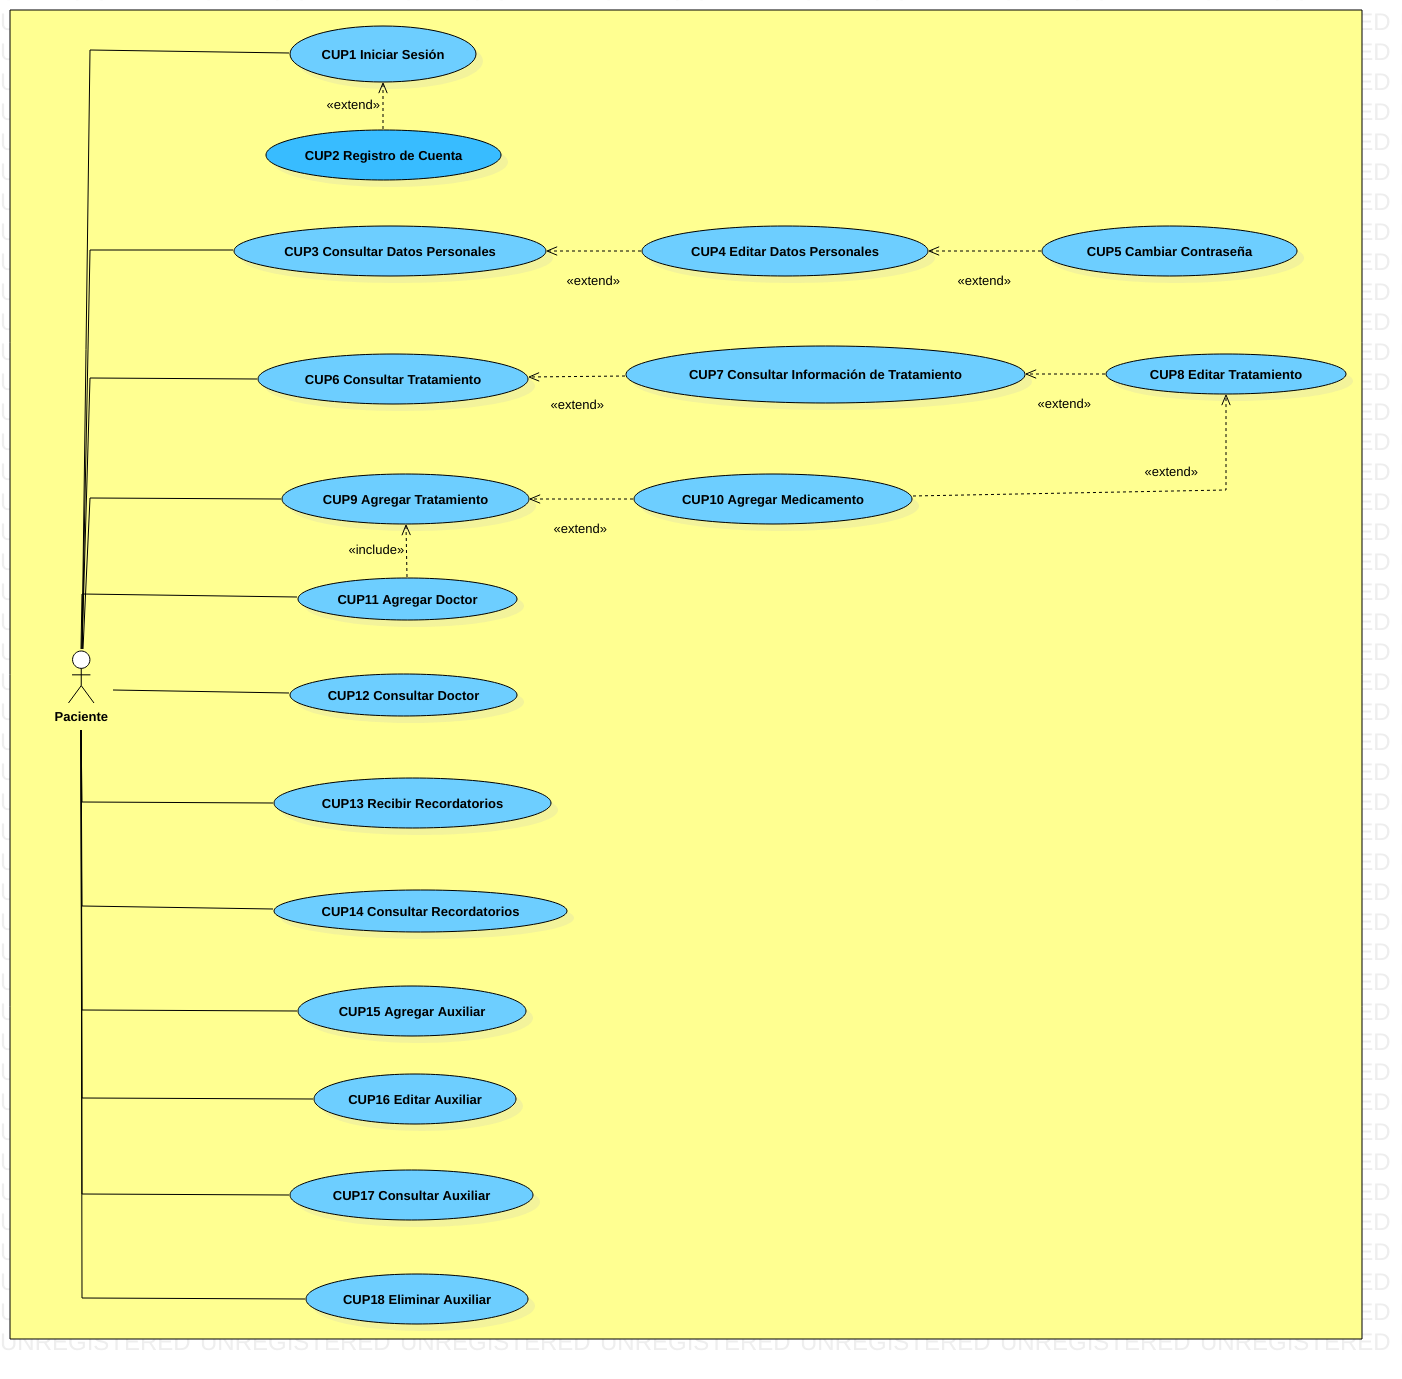
\includegraphics[width=1.1\textwidth]{images/cap2/DCUPaciente2}
	\caption{Casos de uso del paciente} \label{fig:casosdeuso}
\end{figure}


\begin{figure}[htb]
	\centering
	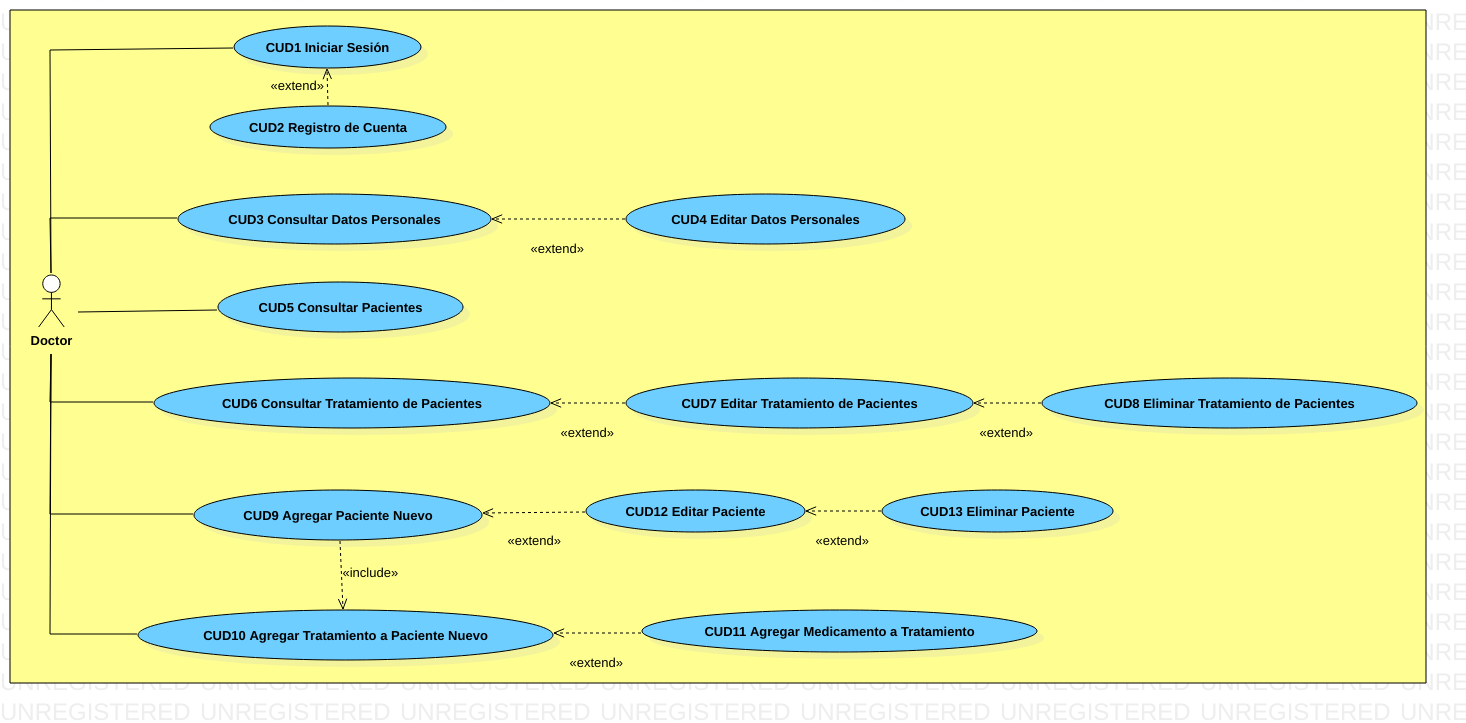
\includegraphics[width=1.1\textwidth]{images/cap2/DCUDoctor2}
	\caption{Casos de uso del Doctor} \label{fig:casosdeusoD}
\end{figure}

\begin{figure}[htb]
	\centering
	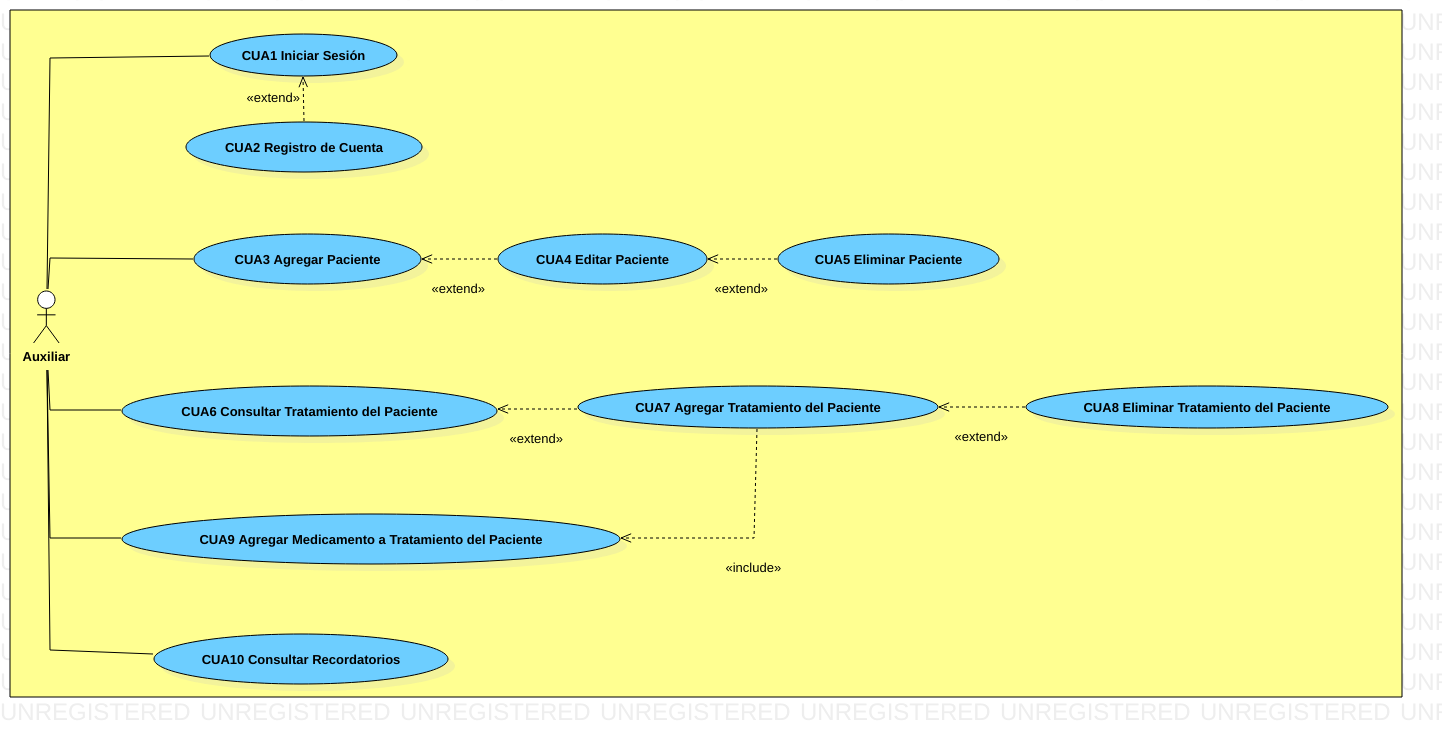
\includegraphics[width=1.1\textwidth]{images/cap2/DCUAuxiliar2}
	\caption{Casos de uso del Auxiliar} \label{fig:casosdeusoA}
\end{figure}

La aplicación con el rol del Paciente cuenta con los siguientes casos de uso:

\begin{itemize}
	\item Paciente:
	\begin{itemize}
		\item CUP1: Iniciar Sesión
		%			\item CUP2: Recuperar Contraseña
		\item CUP2: Registro de Cuenta
		\item CUP3: Consultar Datos Personales
		\item CUP4: Editar Datos Personales
		\item CUP5: Cambiar Contraseña
		\item CUP6: Consultar Tratamiento
		\item CUP7: Consultar Información de Tratamiento
		\item CUP8: Editar Tratamiento
		\item CUP9: Agregar Tratamiento
		\item CUP10: Agregar Medicamento
		\item CUP11: Agregar Doctor
		%			\item CUP13: Editar Doctor
		%			\item CUP14: Eliminar Doctor
		\item CUP12: Consultar Doctor
		\item CUP13: Recibir Recordatorios
		%			\item CUP17: Mandar Alerta
		\item CUP14: Consultar Recordatorios
		%			\item CUP19: Consultar Alertas
		\item CUP15: Agregar Auxiliar
		\item CUP16: Editar Auxiliar
		\item CUP17: Consultar Auxiliar
		\item CUP18: Eliminar Auxiliar
		%			\item CUP24: Agregar Contacto de Emergencia
		%			\item CUP25: Editar Contacto de Emergencia
		%			\item CUP26: Consultar Contacto de Emergencia
		%			\item CUP27: Eliminar Contacto de Emergencia
	\end{itemize}

	
La aplicación con el rol del Doctor cuenta con los siguientes casos de uso:	 
	
		\item Doctor:
	\begin{itemize}
		
		\item CUD1: Iniciar Sesión
		%			\item CUD2: Recuperar Contraseña
		\item CUD2: Registro de Cuenta
		%			\item CUD4: Registrar Datos Personales
		\item CUD3: Consultar Datos Personales
		\item CUD4: Editar Datos Personales
		\item CUD5: Consultar Pacientes
		\item CUD6: Consultar Tratamiento de Pacientes
		\item CUD7: Editar Tratamiento de Pacientes
		\item CUD8: Eliminar Tratamiento de Pacientes
		\item CUD9: Agregar Paciente Nuevo
		\item CUD10: Agregar Tratamiento a Paciente Nuevo
		\item CUD11: Agregar Medicamento a Tratamiento
		\item CUD12: Editar Paciente
		\item CUD13: Eliminar Paciente
		%			\item CUD15: Consultar Historial Clínico
		
	\end{itemize}
	
La aplicación con el rol del Auxiliar cuenta con los siguientes casos de uso:
	
	\item Auxiliar:
		\begin{itemize}
		
		
		\item CUA1: Iniciar Sesión
		%			\item CUA2: Recuperar Contraseña
		\item CUA2: Registro de Cuenta
		\item CUA3: Agregar Paciente
		\item CUA4: Editar Paciente
		\item CUA5: Eliminar Paciente
		\item CUA6: Consultar Tratamiento del Paciente
		\item CUA7: Agregar Tratamiento del Paciente
		\item CUA8: Eliminar Tratamiento del Paciente
		\item CUA9: Agregar Medicamento a Tratamiento del Paciente
		%			\item CUA11: Consultar Contactos de Emergencia
		%			\item CUA12: Agregar Contactos de Emergencia
		%			\item CUA13: Eliminar Contactos de Emergencia
		\item CUA10: Consultar Recordatorios
		%			\item CUA15: Consultar Alertas
			
		\end{itemize}
	

	
\end{itemize}


\chapter{Modelo de Comportamiento del Paciente: Casos de Uso del paciente \label{chp:modeloComportamientoPaciente}}
\newpage
En este capítulo se describen los casos de uso referentes a las acciones que tendrá el rol del Paciente dentro de la aplicación Rem-Pills. \bigskip

\begin{objetivos}[Elementos de un caso de uso]
	\item {\bf Resumen:} Descripción textual del caso de uso.
	\item {\bf Actores:} Lista de los actores que intervienen en el caso de uso.
	\item {\bf Propósito:} Una breve descripción del objetivo que busca el actor al ejecutar el caso de uso.
	\item {\bf Entradas:} Lista de los datos de entrada requeridos durante la ejecución del caso de uso.
	\item {\bf Salidas:} Lista de los datos de salida que presenta el sistema durante la ejecución del caso de uso.
	\item {\bf Precondiciones:} Descripción de las operaciones o condiciones que se deben cumplir previamente para que el caso de uso pueda ejecutarse correctamente.
	\item {\bf Postcondiciones:} Lista de los cambios que ocurrirán en el sistema después de la ejecución del caso de uso y de las consecuencias en el sistema.
	\item {\bf Reglas de negocio:} Lista de las reglas que describen, limitan o controlan algún aspecto del negocio del caso de uso.
	\item {\bf Mensajes:} Lista de los posibles mensajes que pueden surgir durante la ejecución del caso de uso.
	\item {\bf Trayectorias:} Secuencia de los pasos que ejecutará el caso de uso.
\end{objetivos}
%
\cfinput{ModeloPaciente/cup1/uc}
%\cfinput{ModeloPaciente/cup2/uc}
\cfinput{ModeloPaciente/cup3/uc} %%cup2 Registro de cuenta
\cfinput{ModeloPaciente/cup4/uc} %%cup3 Consultar Datos
\cfinput{ModeloPaciente/cup5/uc} %%cup4 Editar Datos
\cfinput{ModeloPaciente/cup6/uc} %%cup5 Cambiar contraseña
\cfinput{ModeloPaciente/cup7/uc} %%cup6 Consultar tratamiento
\cfinput{ModeloPaciente/cup8/uc} %%cup7 Consultar informacion tratamiento
\cfinput{ModeloPaciente/cup9/uc} %%cup8 Editar tratamiento
\cfinput{ModeloPaciente/cup10/uc} %%cup9 Agregar Tratamiento
\cfinput{ModeloPaciente/cup11/uc} %%cup10 Agregar Medicamento
\cfinput{ModeloPaciente/cup12/uc} %%cup11 Agregar doctor
%\cfinput{ModeloPaciente/cup13/uc}
%\cfinput{ModeloPaciente/cup14/uc}
\cfinput{ModeloPaciente/cup15/uc} %%cup12 Consultar doctor
\cfinput{ModeloPaciente/cup16/uc} %%cup13 Recibir recordatorios
%\cfinput{ModeloPaciente/cup17/uc}
\cfinput{ModeloPaciente/cup18/uc} %%cup14 Consultar recordatorios
%\cfinput{ModeloPaciente/cup19/uc}
\cfinput{ModeloPaciente/cup20/uc} %%cup15 Agregar auxiliar
\cfinput{ModeloPaciente/cup21/uc} %%cup16 Editar auxiliar
\cfinput{ModeloPaciente/cup22/uc} %%cup17 Consultar auxiliar
\cfinput{ModeloPaciente/cup23/uc} %%cup18 Elimiar auxiliar
%\cfinput{ModeloPaciente/cup24/uc}
%\cfinput{ModeloPaciente/cup25/uc}
%\cfinput{ModeloPaciente/cup26/uc}
%\cfinput{ModeloPaciente/cup27/uc}
\newpage
%%%%%%%%%%%%%%%%%%%%%%%%%%%%%%%%%%%%%%%%%%%%%%%%
\chapter{Modelo de Comportamiento del Doctor: Casos de Uso del doctor \label{chp:modeloComportamientoDoctor}}

\newpage
En este capítulo se describen los casos de uso referentes a las acciones que tendrá el rol del Doctor dentro de la aplicación Rem-Pills. \bigskip

\begin{objetivos}[Elementos de un caso de uso]
	\item {\bf Resumen:} Descripción textual del caso de uso.
	\item {\bf Actores:} Lista de los actores que intervienen en el caso de uso.
	\item {\bf Propósito:} Una breve descripción del objetivo que busca el actor al ejecutar el caso de uso.
	\item {\bf Entradas:} Lista de los datos de entrada requeridos durante la ejecución del caso de uso.
	\item {\bf Salidas:} Lista de los datos de salida que presenta el sistema durante la ejecución del caso de uso.
	\item {\bf Precondiciones:} Descripción de las operaciones o condiciones que se deben cumplir previamente para que el caso de uso pueda ejecutarse correctamente.
	\item {\bf Postcondiciones:} Lista de los cambios que ocurrirán en el sistema después de la ejecución del caso de uso y de las consecuencias en el sistema.
	\item {\bf Reglas de negocio:} Lista de las reglas que describen, limitan o controlan algún aspecto del negocio del caso de uso.
	\item {\bf Mensajes:} Lista de los posibles mensajes que pueden surgir durante la ejecución del caso de uso.
	\item {\bf Trayectorias:} Secuencia de los pasos que ejecutará el caso de uso.
\end{objetivos}
%
\cfinput{ModeloDoctor/cud1/uc}
%\cfinput{ModeloDoctor/cud2/uc}
\cfinput{ModeloDoctor/cud3/uc} %%cud2 Registro de Cuenta
\cfinput{ModeloDoctor/cud4/uc} %%cud3 Consultar Datos
\cfinput{ModeloDoctor/cud5/uc} %%cud4 Editar Datos
\cfinput{ModeloDoctor/cud6/uc} %%cud5 Consultar Pacientes
\cfinput{ModeloDoctor/cud7/uc} %%cud6 Consultar Tratamiento
\cfinput{ModeloDoctor/cud8/uc} %%cud7 Editar Tratamiento
\cfinput{ModeloDoctor/cud9/uc} %%cud8 ELiminar Tratamiento
\cfinput{ModeloDoctor/cud10/uc} %%cud9 Agregar Paciente
\cfinput{ModeloDoctor/cud11/uc} %%cud10 Agregar Tratamiento
\cfinput{ModeloDoctor/cud12/uc} %%cud11 Agregar Medicamento
\cfinput{ModeloDoctor/cud13/uc} %%cud12 Editar Paciente
\cfinput{ModeloDoctor/cud14/uc} %%cud13 Eliminar Paciente
%\cfinput{ModeloDoctor/cud15/uc}

%
%
%%%%%%%%%%%%%%%%%%%%%%%%%%%%%%%%%%%%%%%%%%%%%%%%%%%
\chapter{Modelo de Comportamiento del Auxiliar: Casos de Uso del auxiliar \label{chp:modeloComportamientoAuxiliar}}
%%En este capítulo se describen los casos de uso referentes al registro y modificación de la información de las escuelas y del comité asociado a cada una de ellas. \bigskip
\newpage
En este capítulo se describen los casos de uso referentes a las acciones que tendrá el rol del Auxiliar dentro de la aplicación Rem-Pills. \bigskip

\begin{objetivos}[Elementos de un caso de uso]
	\item {\bf Resumen:} Descripción textual del caso de uso.
	\item {\bf Actores:} Lista de los actores que intervienen en el caso de uso.
	\item {\bf Propósito:} Una breve descripción del objetivo que busca el actor al ejecutar el caso de uso.
	\item {\bf Entradas:} Lista de los datos de entrada requeridos durante la ejecución del caso de uso.
	\item {\bf Salidas:} Lista de los datos de salida que presenta el sistema durante la ejecución del caso de uso.
	\item {\bf Precondiciones:} Descripción de las operaciones o condiciones que se deben cumplir previamente para que el caso de uso pueda ejecutarse correctamente.
	\item {\bf Postcondiciones:} Lista de los cambios que ocurrirán en el sistema después de la ejecución del caso de uso y de las consecuencias en el sistema.
	\item {\bf Reglas de negocio:} Lista de las reglas que describen, limitan o controlan algún aspecto del negocio del caso de uso.
	\item {\bf Mensajes:} Lista de los posibles mensajes que pueden surgir durante la ejecución del caso de uso.
	\item {\bf Trayectorias:} Secuencia de los pasos que ejecutará el caso de uso.
\end{objetivos}

\cfinput{ModeloAuxiliar/cua1/uc}
%\cfinput{ModeloAuxiliar/cua2/uc}
\cfinput{ModeloAuxiliar/cua3/uc} %%cua2 Registro de cuenta
\cfinput{ModeloAuxiliar/cua4/uc} %%cua3 Agregar Paciente
\cfinput{ModeloAuxiliar/cua5/uc} %%cua4 Editar Paciente
\cfinput{ModeloAuxiliar/cua6/uc} %%cua5 Eliminar Paciente
\cfinput{ModeloAuxiliar/cua7/uc} %%cua6 Consultar Tratamiento
\cfinput{ModeloAuxiliar/cua8/uc} %%cua7 Agregar tratamiento
\cfinput{ModeloAuxiliar/cua9/uc} %%cua8 Eliminar Tratamiento
\cfinput{ModeloAuxiliar/cua10/uc} %%cua9 Agregar Medicamento
%\cfinput{ModeloAuxiliar/cua11/uc}
%\cfinput{ModeloAuxiliar/cua12/uc}
%\cfinput{ModeloAuxiliar/cua13/uc}
\cfinput{ModeloAuxiliar/cua14/uc} %%cua10 Consultar Recordatorios
%\cfinput{ModeloAuxiliar/cua15/uc}
%
\newpage
\chapter{Interfaces del sistema}
\section{Interfaces del sistema: Paciente}
\cfinput{ModeloPaciente/cup1/ui}
%\cfinput{ModeloPaciente/cup2/ui}
\cfinput{ModeloPaciente/cup3/ui} %%iup2
\cfinput{ModeloPaciente/cup4/ui} %%iup3
\cfinput{ModeloPaciente/cup5/ui} %%iup4
\cfinput{ModeloPaciente/cup6/ui} %%iup5
\cfinput{ModeloPaciente/cup7/ui} %%iup6
\cfinput{ModeloPaciente/cup8/ui} %%iup7
\cfinput{ModeloPaciente/cup9/ui} %%iup8
\cfinput{ModeloPaciente/cup10/ui} %%iup9
\cfinput{ModeloPaciente/cup11/ui} %%iup10
\cfinput{ModeloPaciente/cup12/ui} %%iup11
%\cfinput{ModeloPaciente/cup13/ui}
%\cfinput{ModeloPaciente/cup14/ui}
\cfinput{ModeloPaciente/cup15/ui} %%iup12
\cfinput{ModeloPaciente/cup16/ui} %%iup13
%\cfinput{ModeloPaciente/cup17/ui}
\cfinput{ModeloPaciente/cup18/ui} %%iup14
%\cfinput{ModeloPaciente/cup19/ui}
\cfinput{ModeloPaciente/cup20/ui} %%iup15
\cfinput{ModeloPaciente/cup21/ui} %%iup16
\cfinput{ModeloPaciente/cup22/ui} %%iup17
\cfinput{ModeloPaciente/cup23/ui} %%iup18
%\cfinput{ModeloPaciente/cup24/ui}
%\cfinput{ModeloPaciente/cup25/ui}
%\cfinput{ModeloPaciente/cup26/ui}
%\cfinput{ModeloPaciente/cup27/ui}

\section{Interfaces del sistema: Doctor}
\cfinput{ModeloDoctor/cud1/ui}
\cfinput{ModeloDoctor/cud3/ui} 
\cfinput{ModeloDoctor/cud4/ui} 
\cfinput{ModeloDoctor/cud5/ui} 
\cfinput{ModeloDoctor/cud6/ui} 
\cfinput{ModeloDoctor/cud7/ui} 
\cfinput{ModeloDoctor/cud8/ui} 
\cfinput{ModeloDoctor/cud9/ui}
\cfinput{ModeloDoctor/cud10/ui}
\cfinput{ModeloDoctor/cud11/ui}
\cfinput{ModeloDoctor/cud12/ui}
\cfinput{ModeloDoctor/cud13/ui}
\cfinput{ModeloDoctor/cud14/ui}

\section{Interfaces del sistema: Auxiliar}
\cfinput{ModeloAuxiliar/cua1/ui}
\cfinput{ModeloAuxiliar/cua3/ui}
\cfinput{ModeloAuxiliar/cua4/ui}
\cfinput{ModeloAuxiliar/cua5/ui}
\cfinput{ModeloAuxiliar/cua6/ui}
\cfinput{ModeloAuxiliar/cua7/ui}
\cfinput{ModeloAuxiliar/cua8/ui}
\cfinput{ModeloAuxiliar/cua9/ui}
\cfinput{ModeloAuxiliar/cua10/ui}
\cfinput{ModeloAuxiliar/cua14/ui}

%

\chapter{Modelo de Interacción}
\section{Modelo de Interacción}

\cfinput{ModeloInteraccion/mensajes}

\chapter{Modelo de Negocios}
\section{Modelo de Negocios}

\cfinput{ModeloNegocios/reglas}
